%\PassOptionsToPackage{dvipsnames}{xcolor}
\documentclass[tikz,border=5pt]{standalone}
\usetikzlibrary{decorations.text}
\usepackage{libertineotf}
\usepackage{yfonts}
\usepackage{soul}

\begin{document}


\definecolor{myblau}{HTML}{bdbcbc}%00adef}
 


\newcommand{\obere}{
  |  \Large| Αἰών | \Large|παίς | \Large |ἔστι | \Large |παίζων, |\Large|πεσσεύων·  
}



\newcommand{\untere}{
   | \Large| παιδὸς | \Large | ἡ | \Large |  βασιλῄη 
}


\begin{tikzpicture}
\begin{scope}
\draw[color=gray,fill=myblau] (0,0) circle (3.3cm);
\draw[color=gray,fill=white] (0,0) circle (2.6cm);
\end{scope}
\draw[color=gray] (0,0) circle (3.4cm);
\draw[color=gray] (0,0) circle (2.5cm) node {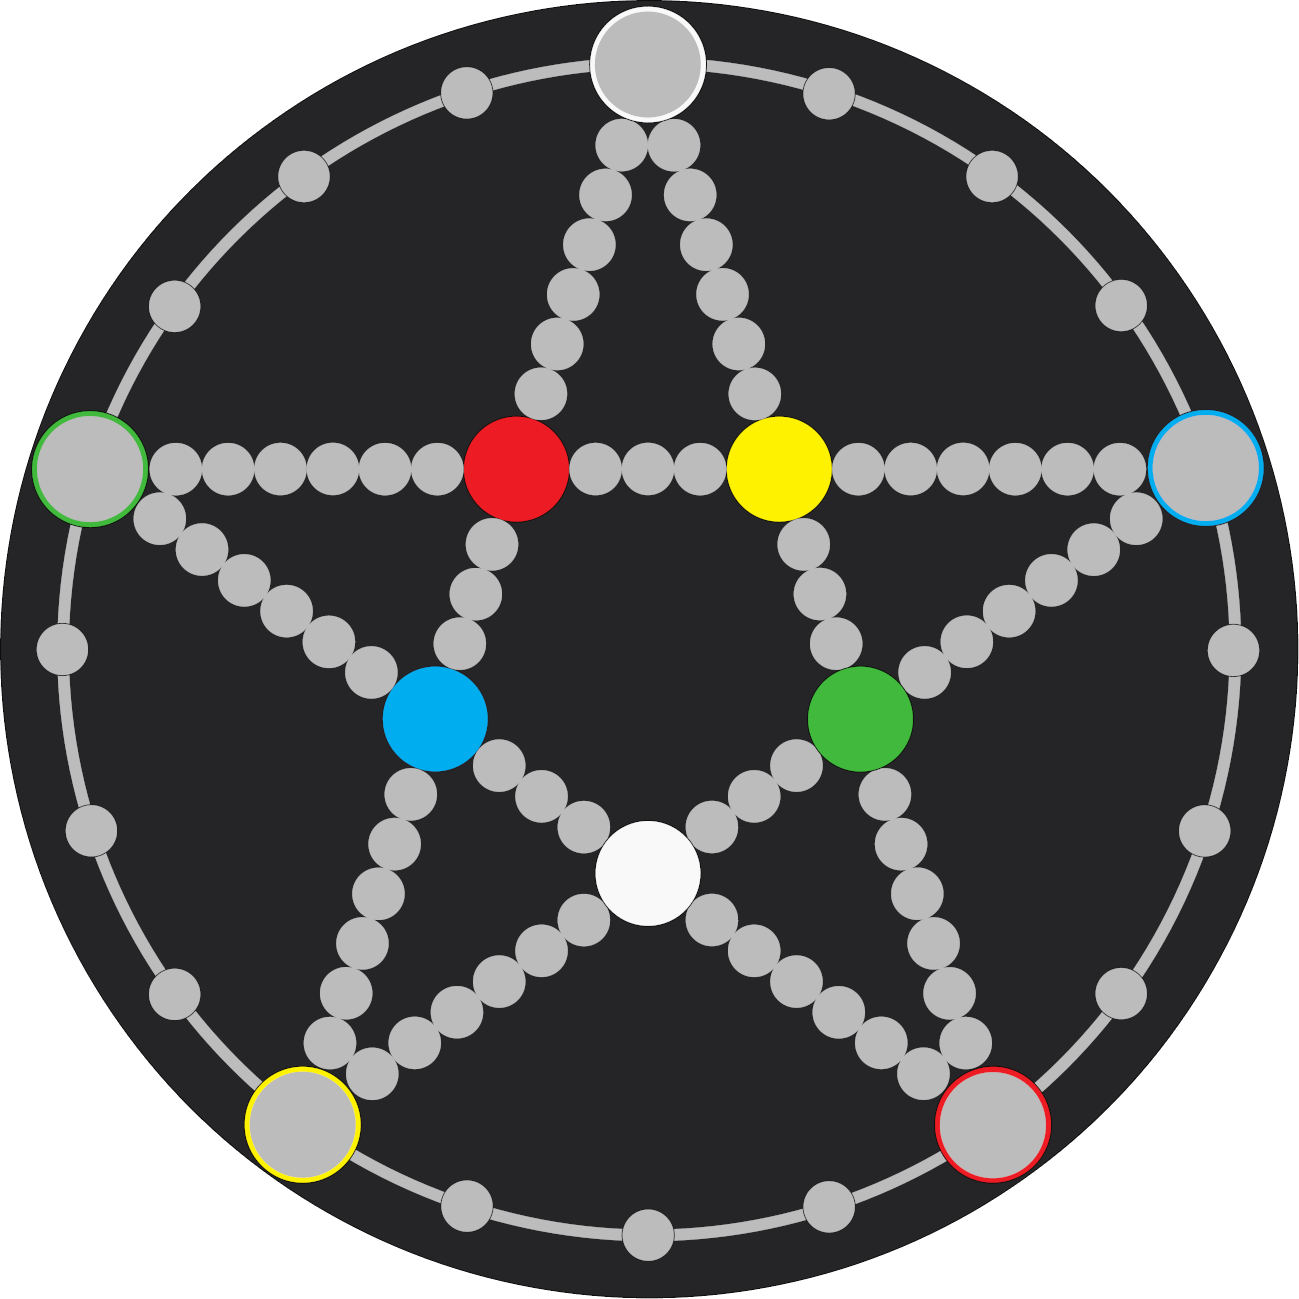
\includegraphics[width=5cm]{Pentagame-board-nob-trans.png}};

\path
    [
        postaction={
            decorate,
            decoration={
                raise=-7pt,
                text along path,
                text align/fit to path stretching spaces=true,
                reverse path=true,
                text align/align=center,
                text align/left indent={9.5818575934488693773110623190025cm}, % \pi * radius
                text align/right indent={0.0cm},
                text={\obere  }
            }
        }
    ]
    [
        postaction={
            decorate,
            decoration={
                raise=-0.5pt,
                text along path,
%               text align/fit to path stretching spaces=true,
%               reverse path=true,
                text align/align=center,
                text align/left indent={9.7818575934488693773110623190025cm}, % \pi * radius + .2cm
                text align/right indent={0.4cm},
                text={| \bfseries\huge | \untere}
            }
        }
    ]
(0,0) circle (3.05cm);
\end{tikzpicture}
\end{document}